% $Header: /cvsroot/latex-beamer/latex-beamer/solutions/conference-talks/conference-ornate-20min.en.tex,v 1.6 2004/10/07 20:53:08 tantau Exp $

\documentclass{beamer}

\mode<presentation>
{
%  \usetheme{Hannover}
\usetheme[width=0.7in]{Hannover}
% or ...

  \setbeamercovered{transparent}
  % or whatever (possibly just delete it)
}
\usepackage{longtable}
\usepackage{booktabs}
\usepackage{qtree}
\usepackage{multicol}

\usepackage[english]{babel}
% or whatever

\usepackage[latin1]{inputenc}
% or whatever
\usepackage{color}

\usepackage{times}
%\usepackage[T1]{fontenc}
% Or whatever. Note that the encoding and the font should match. If T1
% does not look nice, try deleting the line with the fontenc.
%\usepackage{logictheme}

%\usepackage{hhline}
\usepackage{multirow}
%\usepackage{multicol}
%\usepackage{array}
%\usepackage{supertabular}
%\usepackage{amsmath}
%\usepackage{amsfonts}
\usepackage{totpages}
\usepackage{hyperref}
%\usepackage{booktabs}

%\usepackage{bm}

\usepackage{listings}
\usepackage{tikz}
\newcommand{\blt}{- } %used for bullets in a list

\newcounter{datadefnum} %Datadefinition Number
\newcommand{\ddthedatadefnum}{DD\thedatadefnum}
\newcommand{\ddref}[1]{DD\ref{#1}}

\newcommand{\colAwidth}{0.2\textwidth}
\newcommand{\colBwidth}{0.73\textwidth}

\renewcommand{\arraystretch}{0.6} %so that tables with equations do not look crowded

\pgfdeclareimage[height=0.7cm]{logo}{McMasterLogo}
\title[\pgfuseimage{logo}]  % (optional, use only with long paper titles)
{The Drasil Framework}

%\subtitle
%{Include Only If Paper Has a Subtitle}

\author[Slide \thepage~of \pageref{TotPages}] % (optional, use only with lots of
                                              % authors)
{Dan Szymczak}
% - Give the names in the same order as the appear in the paper.
% - Use the \inst{?} command only if the authors have different
%   affiliation.

\institute[McMaster University] % (optional, but mostly needed)
{
  Computing and Software Department\\
  Faculty of Engineering\\
  McMaster University
}
% - Use the \inst command only if there are several affiliations.
% - Keep it simple, no one is interested in your street address.

\date[Jan 24, 2018] % (optional, should be abbreviation of conference name)
{Ernie Mileta Visit, Jan.\ 24, 2018}
% - Either use conference name or its abbreviation.
% - Not really informative to the audience, more for people (including
%   yourself) who are reading the slides online

\subject{computational science and engineering, software engineering, software
  quality, literate programming, software requirements specification, document
  driven design}
% This is only inserted into the PDF information catalog. Can be left
% out. 

% If you have a file called "university-logo-filename.xxx", where xxx
% is a graphic format that can be processed by latex or pdflatex,
% resp., then you can add a logo as follows:

%\pgfdeclareimage[height=0.5cm]{Mac-logo}{McMasterLogo}
%\logo{\pgfuseimage{Mac-logo}}

% Delete this, if you do not want the table of contents to pop up at
% the beginning of each subsection:
\AtBeginSubsection[]
{
  \begin{frame}<beamer>
    \frametitle{Outline}
    \tableofcontents[currentsection,currentsubsection]
  \end{frame}
}

% If you wish to uncover everything in a step-wise fashion, uncomment
% the following command: 

%\beamerdefaultoverlayspecification{<+->}

\beamertemplatenavigationsymbolsempty 

% have SRS and LP open during the presentation

\begin{document}

%%%%%%%%%%%%%%%%%%%%%%%%%%%%%%%%%%%%%%
\begin{frame}

\titlepage

\end{frame}

%%%%%%%%%%%%%%%%%%%%%%%%%%%%%%%%%%%%%%

\begin{frame}

\frametitle{Overview}
\tableofcontents
% You might wish to add the option [pausesections]

% make like a story - the phases - reason for, why works, advantages
% changing the history a bit to make a more rational narrative

\end{frame}

%%%%%%%%%%%%%%%%%%%%%%%%%%%%%%%%%%%%%%

\section[FTS]{Fully Traceable Software} %DS - Better than LSS?

% \subsection[Important Software Qualities]{Scientific Computing Software
% Qualities}

%%%%%%%%%%%%%%%%%%%%%%%%%%%%%%%%%%%%%%

\begin{frame}

\frametitle{Fully Traceable Software}

\begin{itemize}
\item Motivation
\begin{itemize}
\item Improve verifiability, maintainability and reusability.
\item Save money and time% when managing change.
\end{itemize}
\item One ``source,'' multiple views
\begin{itemize}
\item Requirements%, including or excluding derivations.
\item Design
\item Test Cases
\item Build instructions
\item ...
\end{itemize}
\end{itemize}
\end{frame}

%%%%%%%%%%%%%%%%%%%%%%%%%%%%%%%%%%%%%%

\begin{frame}[label=motivation]

\frametitle{Motivation}
\begin{center}
\begin{tikzpicture}[node distance=5mm]
  \tikzstyle{every node}=[draw,shape=rectangle, rounded corners,
    text width=7em, text centered];
  \node (srs) at (-4,0)         	{Requirements};
  \node (dd) at (-3.5,-1.2)  {\alert<3>{Design}};
  \node (src) at (-3,-2.4) 	{\alert<3>{Code}};
  \node (test) at (-2.5, -3.6)       {\alert<3>{Testing}};
\only<2-3>{\node(change) at (0,0) {Change R1};};
	\alt<2-3>{\draw [gray, ->, line width=2pt] (srs) -- (dd);}
  		{\draw [->, line width=2pt] (srs) -- (dd);}
  	\alt<2-3>{\draw [gray, ->, line width=2pt] (dd) -- (src);}
		{\draw [->, line width=2pt] (dd) -- (src);}
  	\alt<2-3>{\draw [gray, ->, line width=2pt] (src) -- (test);}
  		{\draw [->, line width=2pt] (src) -- (test);}
  \only<2-3>{
	\alt<3>{\draw [gray, ->, line width = 3pt] (srs) -- (change);}
		{\draw [->, line width = 3pt] (srs) -- (change);}
	}
  \only<3>{
	\draw [red, ->, line width = 3pt] (change) -- (dd);
	\draw [red, ->, line width = 3pt] (change) -- (src);
	\draw [red, ->, line width = 3pt] (change) -- (test);
	};
\end{tikzpicture}
\end{center}

\end{frame}

%%%%%%%%%%%%%%%%%%%%%%%%%%%%%%%%%%%%%%

\begin{frame}[fragile]

\frametitle{Motivation} %DS Get a better name for this
\framesubtitle{An ``Anonymous'' Quote}
{\fontsize{8}{10}
%% FILL THIS IN %%
\begin{quotation}
  Last year one of a couple vendors presented results after they tried to update
  an analysis from 40 years ago and because the analysis models are not well
  documented they resulted in different final conclusions which had the
  potential to significantly increase operating costs.  I've had to spend the
  last 3 months going over tracking down the impact of each new assumption in
  turn and testing them against available information to see how the original
  results were achieved.  I've found several design features that were credited
  in the original work but not well explained in one case and assumptions about
  how the software worked that were misleading in another.  Had this information
  been better documented a lot of wasted effort could have been avoided.
\end{quotation}}
\end{frame}

%%%%%%%%%%%%%%%%%%%%%%%%%%%%%%%%%%%%%%

\begin{frame}

\frametitle{Last Time}
\begin{itemize}
\item \textit{Knowledge capture}, \textit{chunks}, and \textit{recipes}
\item Common Knowledge Database
\item Document Language
\item Steve
\item Summer Students Phase 1
\end{itemize}

% Common Knowledge Database
% Steve
% Summer Students (Mk I)
% Document Language -- Make sure to have GlassBR working for this one!


\end{frame}

%%%%%%%%%%%%%%%%%%%%%%%%%%%%%%%%%%%%%%

\begin{frame}

\frametitle{Recap - Knowledge Capture}
\begin{center}
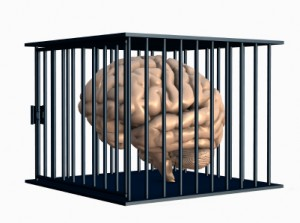
\includegraphics[width=.8\textwidth]{KC.jpg}
\end{center}

\end{frame}

%%%%%%%%%%%%%%%%%%%%%%%%%%%%%%%%%%%%%%

\begin{frame}

\frametitle{Recap - Chunks}

\begin{center}
\includegraphics[width=.8\textwidth]{hierarchy-redesign.png}
\end{center}
%DS This has changed a bit, but new version is too complicated to easily show
% I'll explain that while there are more chunk types, the number of classes
% overall has only increased a bit (Theories, Common Ideas)
\end{frame}

%%%%%%%%%%%%%%%%%%%%%%%%%%%%%%%%%%%%%%

\begin{frame}

\frametitle{Recap - Generation}
\begin{center}

\includegraphics[width=\textwidth]{generate_all_the_things.jpg}
\end{center}

\end{frame}

%%%%%%%%%%%%%%%%%%%%%%%%%%%%%%%%%%%%%%

\begin{frame}

\frametitle{Recap - Drasil}
\begin{center}
	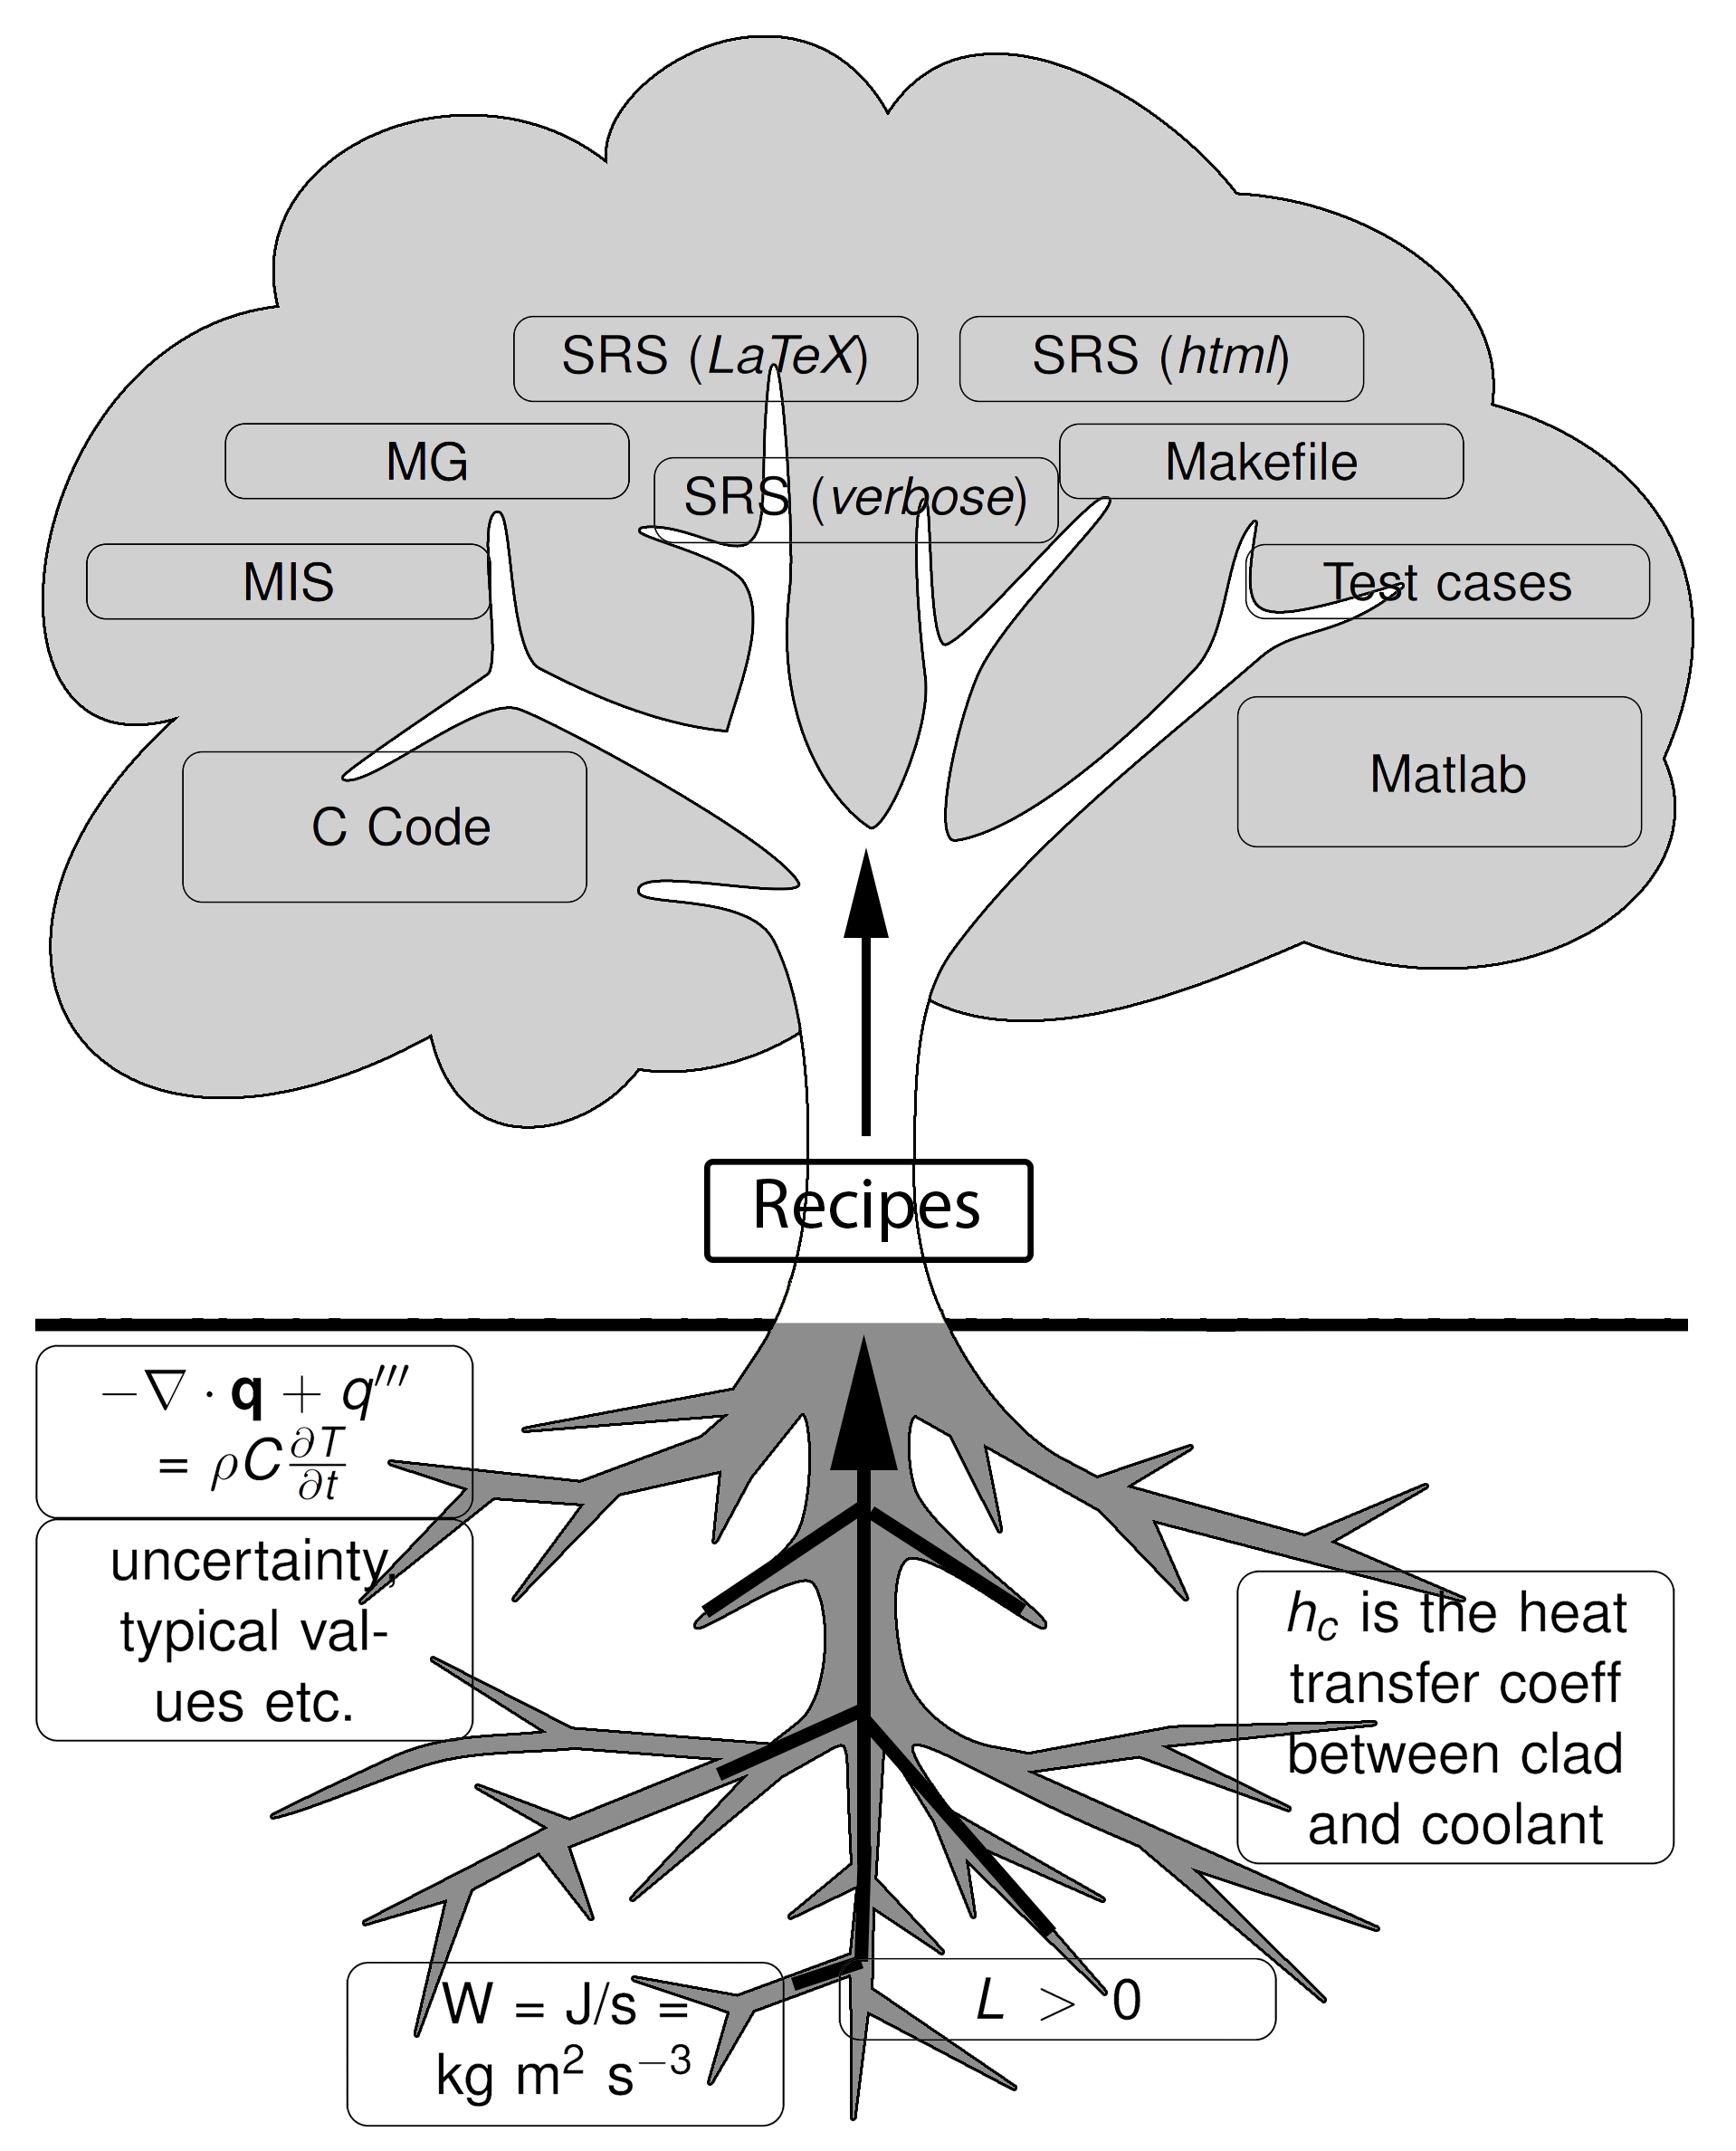
\includegraphics[width=.65\textwidth]{tree.png}
\end{center}

\end{frame}

%%%%%%%%%%%%%%%%%%%%%%%%%%%%%%%%%%%%%%

\section[Drasil]{Drasil Today}

%%%%%%%%%%%%%%%%%%%%%%%%%%%%%%%%%%%%%%

\begin{frame}

\frametitle{What's New}
\framesubtitle{Summer Students Phase 2}

\begin{itemize}
	\item Example clean-up
	\item Knowledge extraction (common + specific)
	\item Pattern finding \& combinator creation
\end{itemize}

\end{frame}

%%%%%%%%%%%%%%%%%%%%%%%%%%%%%%%%%%%%%%

\begin{frame}

\frametitle{What's New}

\framesubtitle{Data.Drasil}

Common Knowledge base expanded! Now includes:
%%% SHOW EXAMPLES HERE
\begin{enumerate}
\item Documentation
\item Thermodynamics 
\item Computation
\item Physics
\item Math
\item Solid Mechanics
\end{enumerate}
and more!

\end{frame}

%%%%%%%%%%%%%%%%%%%%%%%%%%%%%%%%%%%%%%

\begin{frame}

\frametitle{What's New}
\framesubtitle{Continuous Integration}

\begin{center}
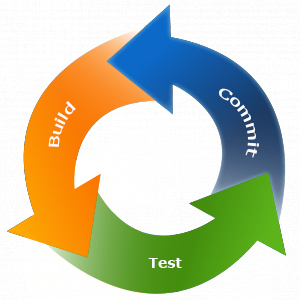
\includegraphics[scale=0.5]{CI.jpg}
\end{center}

\end{frame}

%%%%%%%%%%%%%%%%%%%%%%%%%%%%%%%%%%%%%%

\begin{frame}

\frametitle{What's New}
\framesubtitle{Yuzhi and Devi}

New graduate students as of September 2017.

\begin{itemize}
\item Reviewed and updated manual versions of current examples
\item Implementing Document Language through examples.
\item \ldots{} and more to come!
\end{itemize}

\end{frame}

%%%%%%%%%%%%%%%%%%%%%%%%%%%%%%%%%%%%%%

\begin{frame}

\frametitle{Design Changes}
\framesubtitle{New Knowledge Capture Mechanisms}

We are able to capture much more information in a `useful' form

\begin{enumerate}
	\item Theories
	\item Assumptions
	\item Requirements
	\item Instance Models
\end{enumerate}
...

\end{frame}

%%%%%%%%%%%%%%%%%%%%%%%%%%%%%%%%%%%%%%

%\begin{frame}
%
%\frametitle{Design Changes}
%\framesubtitle{Chunk Hierarchy -- Old}
%
%\large{
%\Tree[.\fbox{Chunk(\textit{name})}
%		[.\fbox{Concept(\textit{description})}
%			[.\fbox{Quantity(\textit{symbol})} ]
%			[.\fbox{Unit(\textit{unit})} ]
%		]
%	]
%}
%\end{frame}

%%%%%%%%%%%%%%%%%%%%%%%%%%%%%%%%%%%%%%

%\begin{frame}
%
%\frametitle{Design Changes}
%\framesubtitle{Chunk Hierarchy -- New}
%
%\begin{center}
%\includegraphics[width=.8\textwidth]{hierarchy-redesign.png}
%\end{center}
%
%\end{frame}

%%%%%%%%%%%%%%%%%%%%%%%%%%%%%%%%%%%%%%

%\begin{frame}
%
%\frametitle{Design Changes}
%\framesubtitle{Abstraction}
%
%\begin{center}
%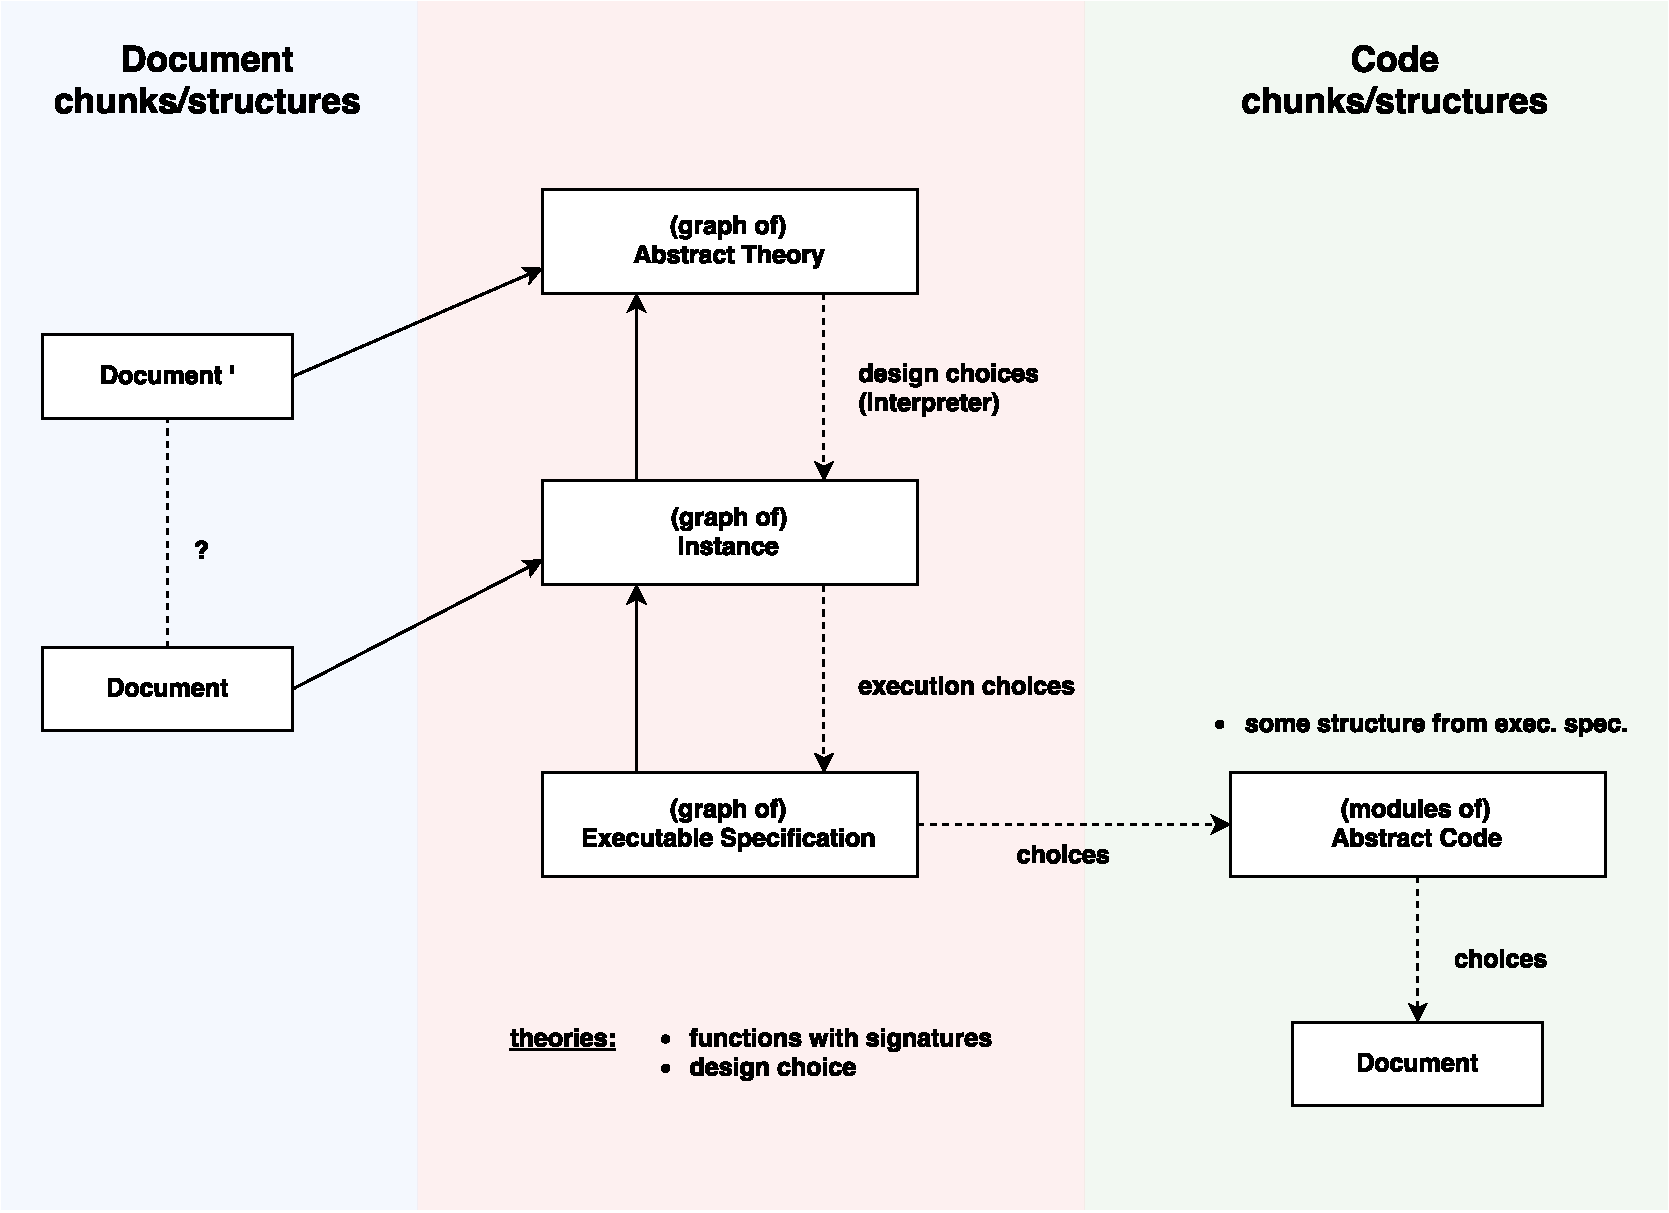
\includegraphics[width=\textwidth]{new_design2.pdf}
%\end{center}
%
%\end{frame}
%
%%%%%%%%%%%%%%%%%%%%%%%%%%%%%%%%%%%%%%

\begin{frame}[fragile]

\frametitle{Design Changes}
\framesubtitle{Document Language -- Old (Recipes)}

\begin{lstlisting}[language=Haskell, frame=single, showstringspaces=false, basicstyle=\scriptsize, escapechar=!]
!\textcolor{blue}{RefSec}! (RefProg intro [
  !\textcolor{red}{TUnits}!, 
  !\textcolor{red}{tsymb''}! s1_2_intro (TermExcept [norm_vect]),
  !\textcolor{red}{TAandA}!]) : 
map Verbatim [s2, s3, s4, s5, s6, s7]

s2 = Section !\ldots{} \ldots{} \ldots{}!
s3 = Section !\ldots{} \ldots{} \ldots{}!
s4 = Section !\ldots{} \ldots{} \ldots{}!
s5 = Section !\ldots{} \ldots{} \ldots{}!
s6 = Section !\ldots{} \ldots{} \ldots{}!
s7 = Section !\ldots{} \ldots{} \ldots{}!

\end{lstlisting} 
%%% EASIER TO WORK WITH / Better understanding of what a recipe should be
\end{frame}

%%%%%%%%%%%%%%%%%%%%%%%%%%%%%%%%%%%%%%

\begin{frame}[fragile]

\frametitle{Design Changes}
\framesubtitle{Document Language -- New (Recipes)}

%DS This is where the section of GlassBR comes into play.
\begin{lstlisting}[language=Haskell, frame=single, showstringspaces=false, basicstyle=\scriptsize, escapechar=!]
!\textcolor{blue}{RefSec}! (RefProg intro 
  [!\textcolor{red}{TUnits}!, !\textcolor{red}{tsymb}! [TSPurpose, SymbOrder], !\textcolor{red}{TAandA}!]) :
!\textcolor{blue}{IntroSec}! ( IntroProg (startIntro ...) (short gLassBR)
  [!\textcolor{red}{IPurpose}! (s2_1_intro_p1 document gLassBR glaSlab),
   !\textcolor{red}{IScope}! incScoR endScoR,
!\ldots{}!
!\textcolor{blue}{GSDSec}! (GSDProg2 [!\textcolor{red}{UsrChars}! ...], !\textcolor{red}{SystCons}! [] []]) :
!\textcolor{blue}{ScpOfProjSec}! (ScpOfProjProg ...) :
!\textcolor{blue}{SSDSec}! (SSDProg
  [!\textcolor{red}{SSDProblem}! (PDProg !\ldots{}! [s6_1_1, s6_1_2, s6_1_3])
  , !\textcolor{red}{SSDSolChSpec}!
    (SCSProg
      [ !\textcolor{red}{TMs}! ([Label] ++ stdFields) [t1IsSafe]
      , !\textcolor{red}{GDs}! [] [] HideDerivation -- No Gen Defs for GlassBR
      , !\textcolor{red}{DDs}! !\ldots{}! , !\textcolor{red}{IMs}! !\ldots{}! ])]) :
!\textcolor{blue}{ReqrmntSec}! (ReqsProg [
  !\textcolor{red}{FReqsSub}! s7_1_list, 
  !\textcolor{red}{NonFReqsSub}! [performance] (gBRpriorityNFReqs) :
!\ldots{}!
!\textcolor{blue}{AuxConstntSec}! (AuxConsProg gLassBR auxiliaryConstants) :
!\textcolor{blue}{Bibliography}! gbCitations :
!\textcolor{blue}{AppndxSec}! (AppndxProg [s12_intro, fig_5, fig_6]) : []
\end{lstlisting}

\end{frame}

%%%%%%%%%%%%%%%%%%%%%%%%%%%%%%%%%%%%%%

\section[Results]{Results}

%%%%%%%%%%%%%%%%%%%%%%%%%%%%%%%%%%%%%%

\begin{frame}[fragile]

\frametitle{Results}
\framesubtitle{Document Language -- New (Recipes)}

GlassBR\_SRS.html

\end{frame}

%%%%%%%%%%%%%%%%%%%%%%%%%%%%%%%%%%%%%%

\begin{frame}[fragile]

\frametitle{Results} %DS Get a better name for this
\framesubtitle{Sanity Checking}

SSP Example (Issue \#348)

\begin{minipage}{.4\linewidth}
\begin{equation}
S_i = \frac{P_i}{FS}
\end{equation}
\end{minipage}%
\begin{minipage}{.4\linewidth}
\begin{equation}
FS = \frac{S_i}{\tau{}_i}
\end{equation}
\end{minipage}

\vspace{.5cm}Where did $\tau{}_i$ come from?\vspace{.3cm}

Were $S_i$ and $P_i$ swapped?


\begin{itemize}
\item $\tau{}_i$ was not defined anywhere in the documents
\item Found with Drasil -- undefined symbols throw errors
\item Equation based on concepts -- symbols automatically retrieved
\end{itemize}

%Original issue was a bit more complicated, but came down to this.

\end{frame}

%%%%%%%%%%%%%%%%%%%%%%%%%%%%%%%%%%%%%%

\begin{frame}[fragile]

\frametitle{Results} %DS Get a better name for this
\framesubtitle{Sanity Checking Cont'd}

\begin{itemize}
\item Stricter (more formalized) approach reveals hidden errors.

\item Fixing these kinds of errors is easy thanks to tool support from Drasil
\end{itemize}

\end{frame}

%%%%%%%%%%%%%%%%%%%%%%%%%%%%%%%%%%%%%%

\begin{frame}[fragile]

\frametitle{Results} %DS Get a better name for this
\framesubtitle{Conceptual Inconsistencies}

Manually created artifacts are human-readable.

Problems arise when attempting to explain things to a machine.

\begin{itemize}
\item What do our artifacts \emph{mean}?
\item What is each section contributing? %(in an artifact) --> New knowledge (assumps, reqs)? Building off previous towards a solution?
\item Why do we organize things a given way?
\item Are models/definitions different? How?
\end{itemize}

Need to be more rigorous!

\end{frame}

%%%%%%%%%%%%%%%%%%%%%%%%%%%%%%%%%%%%%%

\section[Next Steps]{Next Steps}

%%%%%%%%%%%%%%%%%%%%%%%%%%%%%%%%%%%%%%

\begin{frame}

\frametitle{Next Steps}


\begin{Large}
What next?
\end{Large}

\begin{itemize}
\item Recipe language implementation %finish implementing in examples
\item More examples (in new domains) % Speciation?
\item More artifacts  %new recipes -- Module guide
\item Design Language %Steve
\end{itemize}
\end{frame}

%%%%%%%%%%%%%%%%%%%%%%%%%%%%%%%%%%%%%%

\begin{frame}
\begin{center}
\Huge Thank You!
\end{center}
\end{frame}

%%%%%%%%%%%%%%%%%%%%%%%%%%%%%%%%%%%%%%

\end{document}
